\subsection{Definitions}
\begin{itemize}[label=\(\rhd\)]
    \item \textbf{Database (DB)}: A collection of related data
    \item \textbf{Database Management System (DBMS)}: A software package to facilitate the creation/maintenance/querying of databases
    \item \textbf{Database System (DBS)}: DB + DBMS
    \item \textbf{Meta Data}: Information about the structure of the DB
\end{itemize}

\begin{figure}[H]
\centering
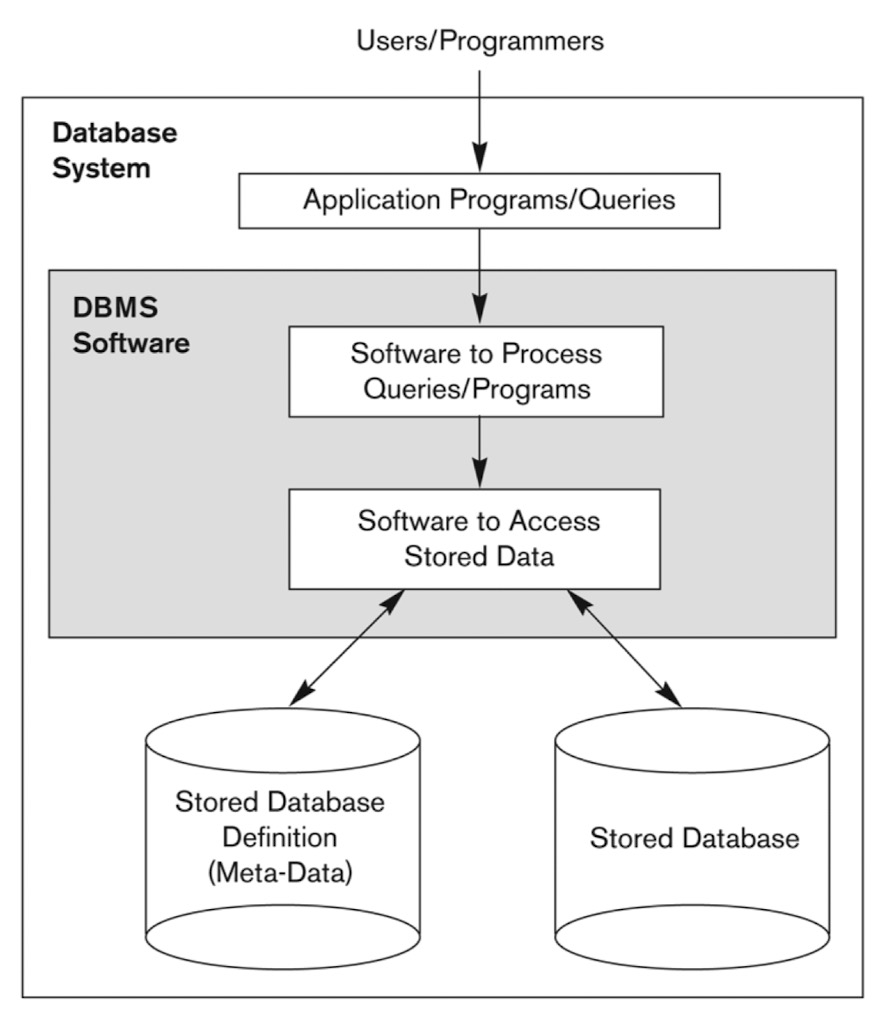
\includegraphics[width=0.8\textwidth]{images/Screenshot 2024-05-01 at 17.02.18.jpg}
\caption{Database System}
\end{figure}

A DBMS offers two types of languages:
\begin{itemize}[label=\(\rhd\)]
    \item[1.] data definition language (\textbf{DDL}) to create and drop tables, etc.
    \item[2.] data manipulation language (\textbf{DML}) to select, insert, delete, and update data 
    \item SQL offers both.
\end{itemize}

\textbf{\underline{Functionality of Database Systems}}
\bigskip
Typical DBMS functionality:
\begin{itemize}[label=\(\rhd\)]
    \item \textbf{Define} a particular database in terms of its data types, structures, and constraints
    \item \textbf{Construct} or \textbf{load} the initial database contents on a persistent storage medium
    \item \textbf{Manipulating} the database:
    \begin{itemize}[label=\(\rhd\)]
        \item Retrieval: querying, generating reports
        \item Modification: insertions, deletions and updates to its content
    \end{itemize}
    \item \textbf{Sharing} by a set of concurrent users and application programs while, at the same time, keeping all data valid and consistent.
\end{itemize}

\textbf{\underline{Redundancy}}
\bigskip
A key goal of database design is to avoid redundancy. \textbf{Redundancy} is present if information is stored multiple times. Redundancy leads to update anomalies and inconsistent data. The term \textbf{controlled redundancy} is used if duplication of information is allowed and if the duplication is controlled by the DBMS.

\subsection{Main Characteristics of Database Systems}

\textbf{\underline{DBMS Architecture}}

\begin{figure}[H]
\centering
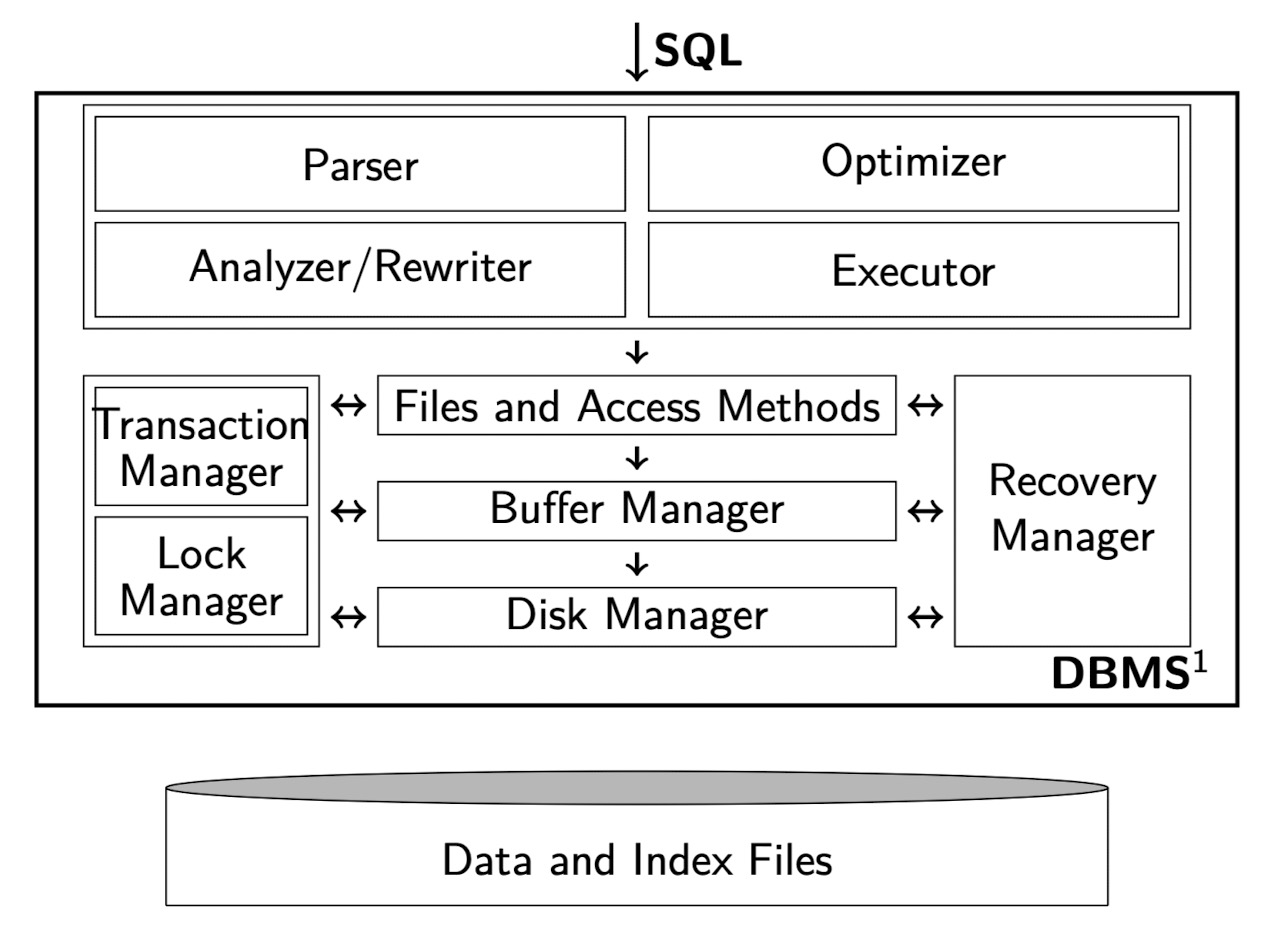
\includegraphics[width=0.8\textwidth]{images/Screenshot 2024-05-01 at 17.25.40.jpg}
\caption{DBMS Architecture}
\end{figure}

\subsection{Summary}
\begin{itemize}[label=\(\rhd\)]
    \item Data models, schema, instances
    \begin{itemize}[label=\(\rhd\)]
        \item \textbf{data model} = structures + constraints + operations
        \item \textbf{schema} = intension; schema consists of structures and constraints; schema changes infrequently 
        \item \textbf{relation instance} = relation = extension; relation instance is the actual data that is compatible with the schema; changes often
    \end{itemize}
    \item Key characteristics of database systems
    \begin{itemize}[label=\(\rhd\)]
        \item \textbf{controlled redundancy}: database systems is aware of redundancy and provides support for updates that could violate the consistency of the data
        \item \textbf{data independence}: separation of program and data; makes it possible to, e.g., reorganize internal schema without changing conceptual schema
        \item \textbf{data abstraction}: high level query language that is independent of storage structure
        \item \textbf{data dictionary} (metadata) that stores information about the database itself (self-describing)
    \end{itemize}
\end{itemize}